\documentclass[10pt]{article}

\usepackage[a4paper,margin=0.65in]{geometry}
\usepackage[utf8]{inputenc}
\usepackage{graphicx}
\usepackage{titlesec}
\usepackage{fancyhdr}
\usepackage{color}
\usepackage{parskip}
\usepackage{helvet}
\usepackage{longtable}
\usepackage{hyperref}
\usepackage{float}
\usepackage{caption}
\usepackage{lastpage}
\usepackage{array}
\usepackage{ragged2e}
\usepackage{makecell}
\usepackage{tabularx}
\usepackage[table]{xcolor}
\usepackage{colortbl}
\usepackage{placeins} % para FloatBarrier

% Colores para tablas
\definecolor{headergray}{gray}{0.9}
\definecolor{rowalt}{RGB}{245,245,255}

% Fuente sans-serif
\renewcommand{\familydefault}{\sfdefault}

% Encabezado
\pagestyle{fancy}
\fancyhf{}
\lhead{
\includegraphics[height=0.7cm]{images/logo_unit.png}}
\rhead{\textbf{PWM module v1.0}}
\lfoot{Product Brief}
\rfoot{\thepage\ | \pageref{LastPage}}

% Estilo de secciones
\titleformat{\section}{\bfseries\large\sffamily}{}{0em}{}
\titleformat{\subsection}{\bfseries\normalsize\sffamily}{}{0em}{}
\titlespacing*{\section}{0pt}{1.2em}{0.5em}
\titlespacing*{\subsection}{0pt}{0.8em}{0.4em}

\title{}
\author{}
\date{}

\sloppy
\setlength{\emergencystretch}{3em}

\begin{document}

% Encabezado del documento
\noindent
\makebox[\textwidth][l]{%
    \begin{minipage}[t]{\textwidth}
        \Large \textbf{PWM module Product Brief}\\[1.0em]
        \normalsize A two-channel PWM module that extends microcontroller PWM signals to drive high-power loads, featuring clearly labeled screw-terminal connectors and a JST 1mm 4 vias header for easy plug-and-play connectivity.\\[0.3em]
        \footnotesize\textsf{Version: 1.0 \hfill Modified: 2025-04-30}
    \end{minipage}%
}
\vspace{1em}
\hrule
\vspace{1.5em}

% Introducción con imagen
\section*{Introduction}
\vspace{0.5em}
\noindent
\begin{minipage}[t]{0.62\textwidth}
\setlength{\parskip}{0.75em}
\justifying
This two-channel PWM module PCB is purpose-built to amplify pulse-width modulation signals from a microcontroller, allowing it to switch external loads at voltages and currents well beyond the device’s native limits. Its compact design, featuring clearly labeled screw-terminal connectors, is ideal for applications such as motor speed control, high-power LED dimming, or any project requiring precise PWM regulation. Additionally, a JST 1mm 4 vias header is included for convenient plug-and-play wiring and daisy-chaining of power and PWM signals.
\end{minipage}
\hfill
\begin{minipage}[t]{0.35\textwidth}
\centering
\vspace{-0.5em}
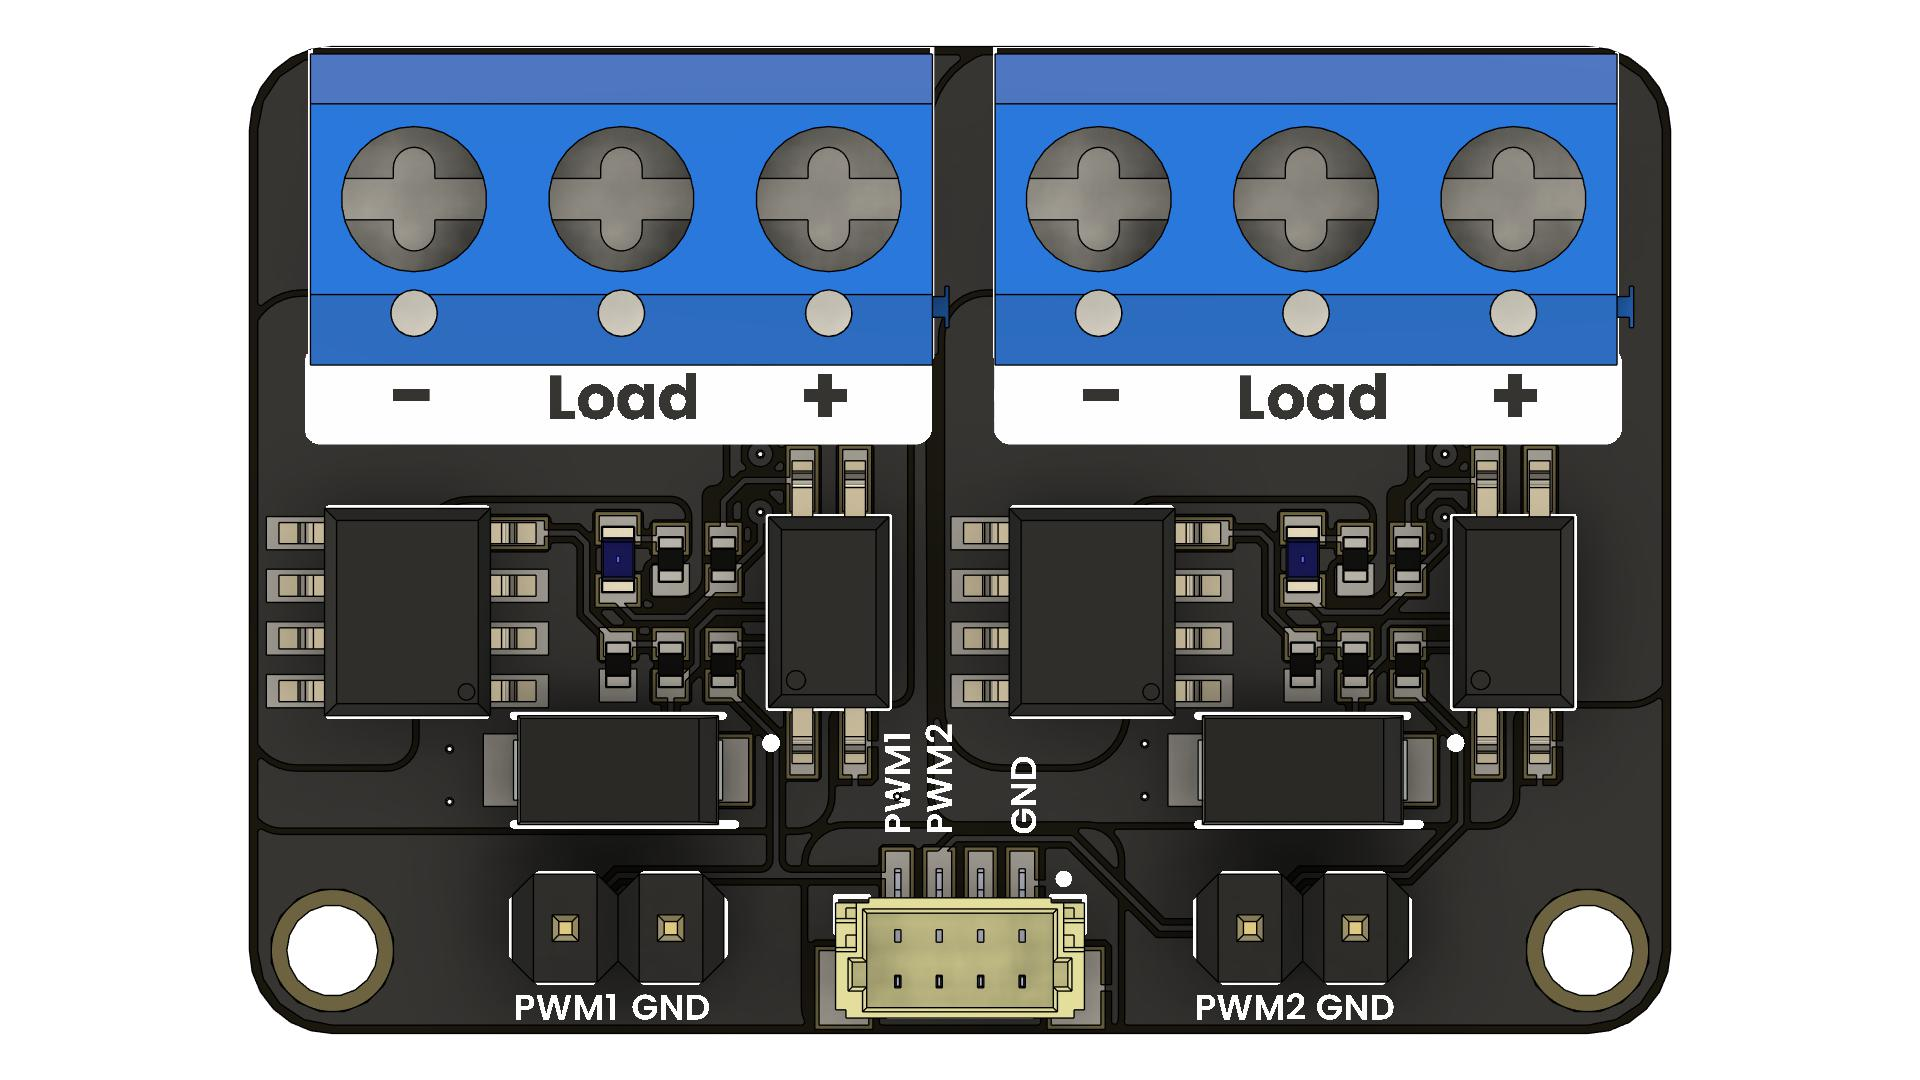
\includegraphics[height=4.5cm,keepaspectratio]{./images/product.jpg}
\end{minipage}

\vspace{1.0em}
\FloatBarrier % evita que la imagen flote sobre el siguiente bloque



% Secciones técnicas
\section*{Functional Description}
- The module is designed to extend the PWM capabilities of microcontrollers, enabling them to control high-power loads such as motors or LEDs.\\ 
- It features two independent channels, each with its own input and output control.\\ 
- The input control accepts PWM signals from the microcontroller, while the output control drives the connected load.\\ 
- The module is equipped with a JST 1mm 4 vias header for easy connection to power and PWM signals.\\ 

\section*{Electrical Characteristics}
-\\ 

\section*{Features}
- The module contains two devices that share the same features but are connected to separate input and output controls, allowing for independent operation.\\ 



\section*{Applications}
- The module is suitable for applications requiring high-power PWM control, such as:\\ 
- Motor speed control\\ 
- High-power LED dimming\\ 
- Any project requiring precise PWM regulation\\ 
- The module can be used in robotics, automation, and other projects where high-power loads need to be controlled with precision.\\ 

\vspace{1em}

\section*{Settings}

\subsection*{Interface Overview}
\rowcolors{2}{white}{rowalt}
\begin{tabularx}{\textwidth}{|c|c|>{\RaggedRight\arraybackslash}X|}
\hline
\rowcolor{headergray}
Interface & Signals / Pins & Typical Use \\
\hline
- & - & - \\
\hline
\end{tabularx}


% Tabla principal
\section*{Pin \& Connector Layout}
\rowcolors{2}{white}{rowalt}
\begin{tabularx}{\textwidth}{|c|c|c|>{\RaggedRight\arraybackslash}X|}
\hline
\rowcolor{headergray}
Device & Input Control & Output Control & Features \\
\hline
PWM 1 & Dedicated input for control & Dedicated output for driving & MOSFET driver with precise control and transient protection \\
PWM 2 & Dedicated input for control & Dedicated output for driving & MOSFET driver with precise control and transient protection \\
\hline
\end{tabularx}


% Imágenes adicionales
\FloatBarrier
\newpage
\vspace*{3em}
\section*{Block Diagram}
\vspace{1em}
\begin{center}
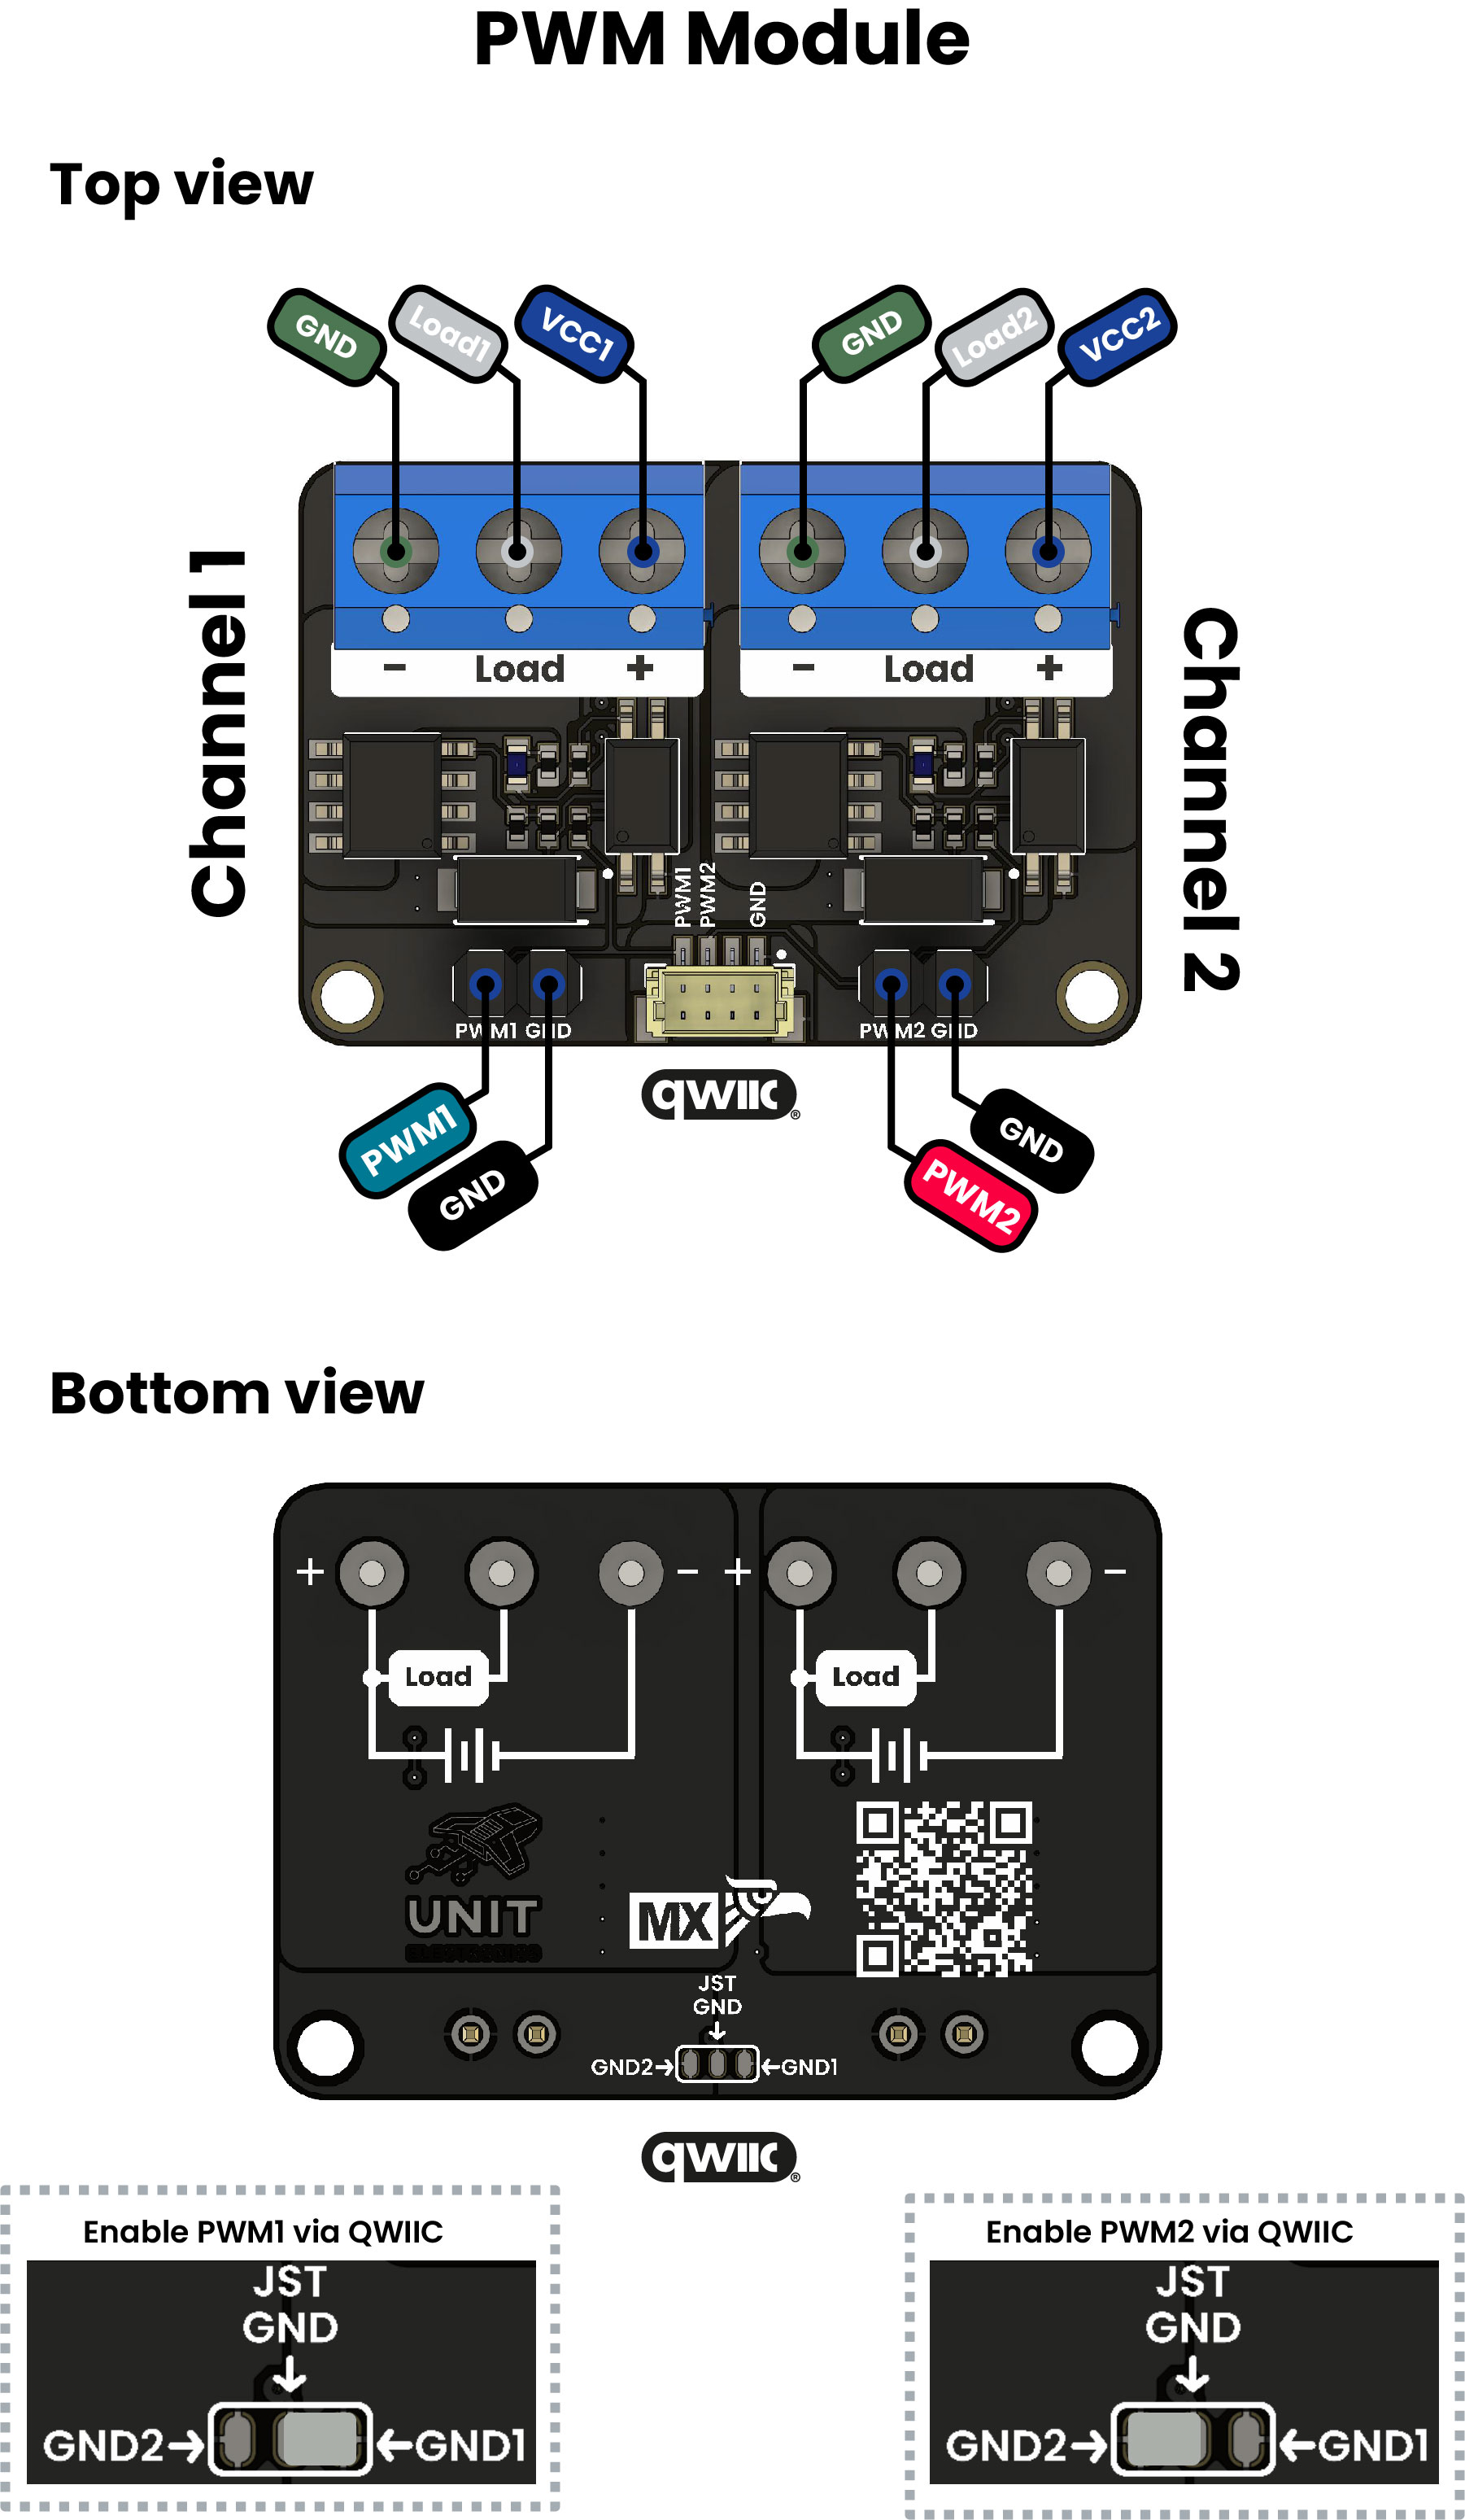
\includegraphics[width=0.70\textwidth,keepaspectratio]{images/function-diagram.jpg}
\end{center}
\newpage
\vspace*{3em}
\section*{Dimensions}
\vspace{1em}
\begin{center}
\includegraphics[width=0.70\textwidth,keepaspectratio]{images/dimensions.png}
\end{center}



% Uso
\section*{Usage}
\begin{itemize}
\item 
\end{itemize}

% Descargas
\section*{Downloads}
\begin{itemize}
\begin{itemize}
\item \href{docs/schematic.pdf}{Schematic PDF}
\end{itemize}
\end{itemize}

% Compra
\section*{Purchase}
\begin{itemize}
\item \href{https://www.uelectronics.com}{Buy from UNIT Electronics}
\end{itemize}

\end{document}
